\documentclass[aspectratio=169]{beamer}
\usepackage{lmodern}
%\usetheme{Madrid}
%\usecolortheme{giantoak}
\newcommand*\oldmacro{}
\let\oldmacro\insertshorttitle
\renewcommand*\insertshorttitle{\oldmacro\hfill\insertframenumber\,/\,\inserttotalframenumber}
\usepackage[framemethod=tikz]{mdframed}

%\usepackage{beamerthemesplit}
\usepackage{textpos}
\usepackage{pgf}
\usepackage{ulem}
%\logo{\pgfputat{\pgfxy(0,-.4)}{\pgfbox[right,base]{\includegraphics[height=1.0cm]{logo.jpg}}}}
%\newcommand{\nologo}{\setbeamertemplate{logo}{}}
\usepackage{booktabs}
\usepackage{graphicx}
\theoremstyle{principle}
\newtheorem*{principle}{Design Principle}


\titlegraphic{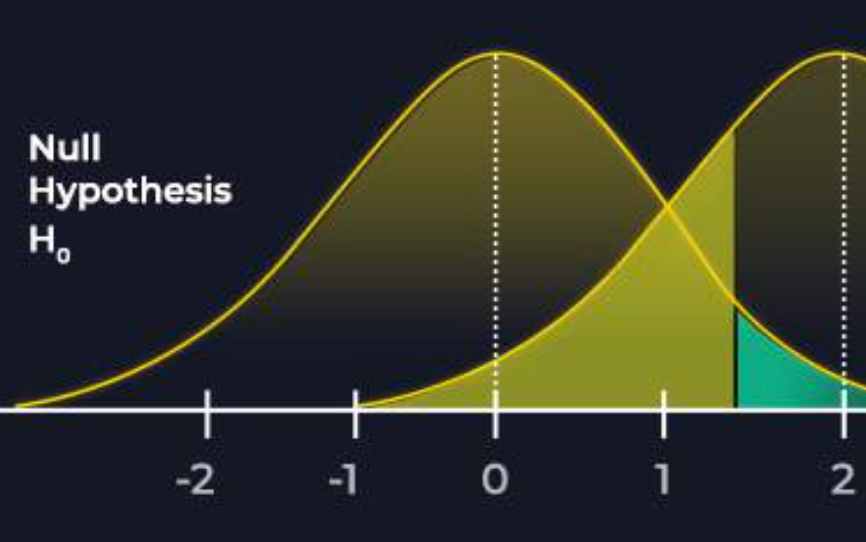
\includegraphics[width=1.0\paperwidth]{distros.png}}

\title{Amendments}
%\author[Jeremy Kedziora]{Wind Data Science Team\\
%\small{Uptake}}
\date{}

\begin{document}

%{
%%\nologo
%\begin{frame}
%    \maketitle
%\end{frame}
%}
%pages 1-7, 8-9, 14-15.


{
%  \usebackgroundtemplate{
\includegraphics[width=1.0\paperwidth]{statistics-review.jpg}}
  \usebackgroundtemplate{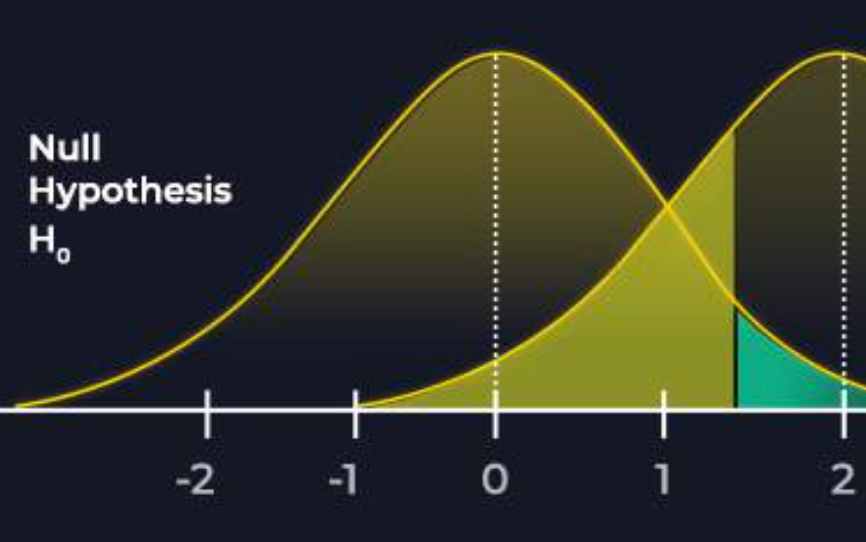
\includegraphics[scale=1.1]{distros.png}}
  \begin{frame}[plain]
  
\begin{mdframed}[tikzsetting={draw=white,fill=white,fill opacity=0.6,draw opacity=0.4,
               line width=0pt},backgroundcolor=none,leftmargin=20,
               rightmargin=20,innertopmargin=4pt]
\begin{center}
\Huge \textbf{Hypothesis Testing}
\end{center}
\end{mdframed}

  \end{frame}
}

%most reliant on human cognition
%limited only by cognition
%hypothesis generating scheme often functioning as a gateway into more statistical analysis

%%@@@@@@@@@@@@@@@@@@@@@@@@@@@@@@@@@@@@@@@@@@@@@@@@@
%\begin{frame}
%\frametitle{Napoleon's Progress}
%\begin{center}
%
\includegraphics[scale=0.4]{experiment.png}
%
\includegraphics[scale=0.35]{stars.png}
%\end{center}
%
%\end{frame}

%@@@@@@@@@@@@@@@@@@@@@@@@@@@@@@@@@@@@@@@@@@@@@@@@@
\begin{frame}
\frametitle{Today:}

\begin{itemize}
\item Define the parts of a hypothesis test;
\bigskip
\bigskip
\bigskip

\item Define $p$-values, understand what they mean, and relate them to type I errors;
\bigskip
\bigskip
\bigskip

\item Work through an example of a hypothesis test in a political context.

\end{itemize}

\end{frame}

%@@@@@@@@@@@@@@@@@@@@@@@@@@@@@@@@@@@@@@@@@@@@@@@@@
\begin{frame}

\begin{center}
\Huge Hypothesis testing is a model that helps us decide between different hypotheses using \textbf{falsification}.\\
\end{center}

\end{frame}

%@@@@@@@@@@@@@@@@@@@@@@@@@@@@@@@@@@@@@@@@@@@@@@@@@
\begin{frame}
\frametitle{Parts of a hypothesis test}

\begin{enumerate}
\item A \textbf{Null hypothesis} $\mathbf{H_0}$;
\begin{itemize}
\item  Usually a claim that there is no effect or nothing of interest;
\item We will be looking to decide if the data falsifies the null hypothesis;
\end{itemize}
\bigskip

\item An \textbf{Alternative hypothesis} $\mathbf{H_A}$;
\begin{itemize}
\item Usually a claim that there IS an effect;
\item We want to create support for this by falsifying its converse;
\end{itemize}
\bigskip

\item[]\color{white} A \textbf{test statistic};
\begin{itemize}
\item[]\color{white} A point estimate summary of the data that we can use to decide between $H_0$ and $H_A$;
\item[]\color{white} Observed test statistic: the actual value of the test stat we observed IRL;
\item[]\color{white} Null distribution: sampling distribution of the test statistic assuming $H_0$  is true;
\end{itemize}
\bigskip

\item[]\color{white} A \textbf{rejection criterion} (also called the significance level);
\begin{itemize}
\item[]\color{white} If we see this happen to the test statistic then we will decide we have falsified or rejected $H_0$;
\item[]\color{white} Largely an arbitrary choice.
\end{itemize}

\end{enumerate}

\end{frame}

%@@@@@@@@@@@@@@@@@@@@@@@@@@@@@@@@@@@@@@@@@@@@@@@@@
\begin{frame}
\frametitle{Parts of a hypothesis test}

\begin{enumerate}
\item A \textbf{Null hypothesis} $\mathbf{H_0}$;
\begin{itemize}
\item  Usually a claim that there is no effect or nothing of interest;
\item We will be looking to decide if the data falsifies the null hypothesis;
\end{itemize}
\bigskip

\item An \textbf{Alternative hypothesis} $\mathbf{H_A}$;
\begin{itemize}
\item Usually a claim that there IS an effect;
\item We want to create support for this by falsifying its converse;
\end{itemize}
\bigskip

\item A \textbf{test statistic};
\begin{itemize}
\item A point estimate summary of the data that we can use to decide between $H_0$ and $H_A$;
\item Observed test statistic: the actual value of the test stat we observed IRL;
\item Null distribution: sampling distribution of the test statistic assuming $H_0$  is true;
\end{itemize}
\bigskip

\item[]\color{white} A \textbf{rejection criterion} (also called the significance level);
\begin{itemize}
\item[]\color{white} If we see this happen to the test statistic then we will decide we have falsified or rejected $H_0$;
\item[]\color{white} Largely an arbitrary choice.
\end{itemize}

\end{enumerate}

\end{frame}

%@@@@@@@@@@@@@@@@@@@@@@@@@@@@@@@@@@@@@@@@@@@@@@@@@
\begin{frame}
\frametitle{Parts of a hypothesis test}

\begin{enumerate}
\item A \textbf{Null hypothesis} $\mathbf{H_0}$;
\begin{itemize}
\item  Usually a claim that there is no effect or nothing of interest;
\item We will be looking to decide if the data falsifies the null hypothesis;
\end{itemize}
\bigskip

\item An \textbf{Alternative hypothesis} $\mathbf{H_A}$;
\begin{itemize}
\item Usually a claim that there IS an effect;
\item We want to create support for this by falsifying its converse;
\end{itemize}
\bigskip

\item A \textbf{test statistic};
\begin{itemize}
\item A point estimate summary of the data that we can use to decide between $H_0$ and $H_A$;
\item Observed test statistic: the actual value of the test stat we observed IRL;
\item Null distribution: sampling distribution of the test statistic assuming $H_0$  is true;
\end{itemize}
\bigskip

\item A \textbf{rejection criterion} (also called the significance level);
\begin{itemize}
\item If we see this happen to the test statistic then we will decide we have falsified or rejected $H_0$;
\item Largely an arbitrary choice.
\end{itemize}

\end{enumerate}

\end{frame}

%@@@@@@@@@@@@@@@@@@@@@@@@@@@@@@@@@@@@@@@@@@@@@@@@@
\begin{frame}
\frametitle{Null distribution}
  
\begin{itemize}
\item \textbf{Remember the marbles in the bag?}  We didn't talk about it but our test statistic was the fraction of blue marbles in the sample;
\bigskip

\item Imagine when we did that our null hypothesis was that the fraction of blue marbles $=$ 66\%.  Then the sampling (null) distribution ought to look like:
\end{itemize}

\begin{center}
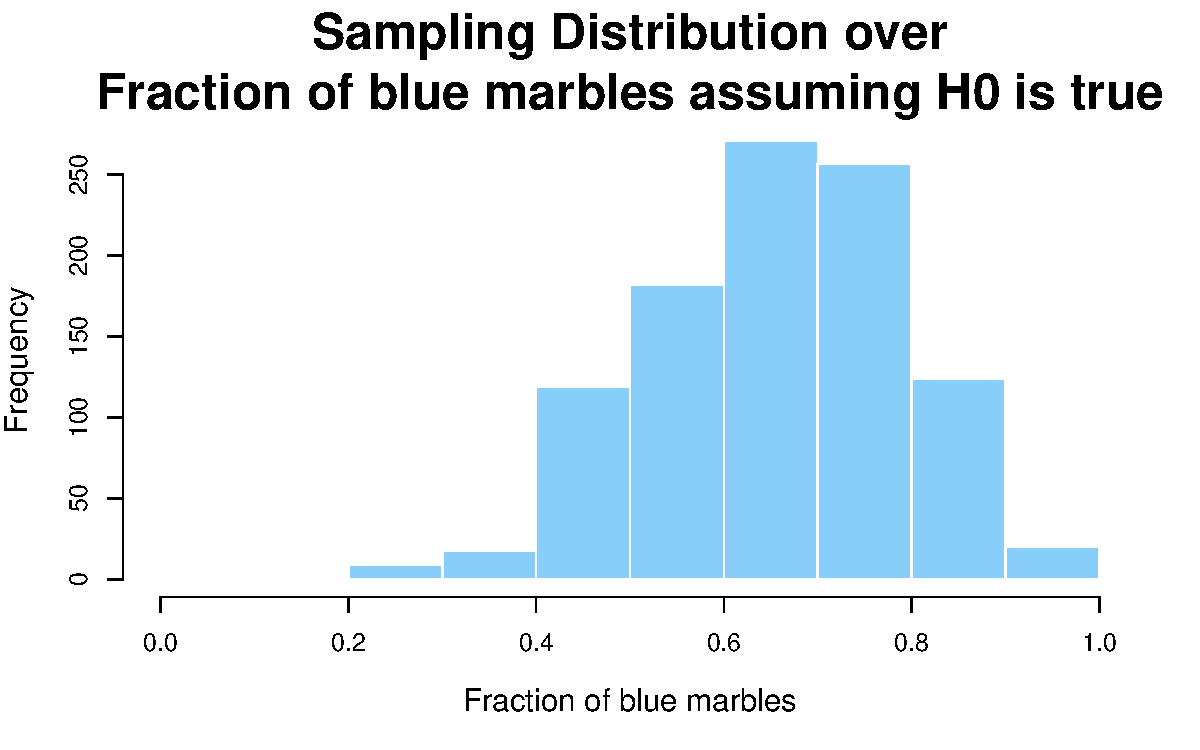
\includegraphics[scale=0.4]{null_66.pdf}
\end{center}

\end{frame}

%@@@@@@@@@@@@@@@@@@@@@@@@@@@@@@@@@@@@@@@@@@@@@@@@@
\begin{frame}
\frametitle{Null distribution}
  
\begin{itemize}
\item \textbf{Remember the marbles in the bag?}  We didn't talk about it but our test statistic was the fraction of blue marbles in the sample;
\bigskip

\item Imagine when we did that our null hypothesis was that the fraction of blue marbles $=$ 50\%.  Then the sampling (null) distribution ought to look like:
\end{itemize}

\begin{center}
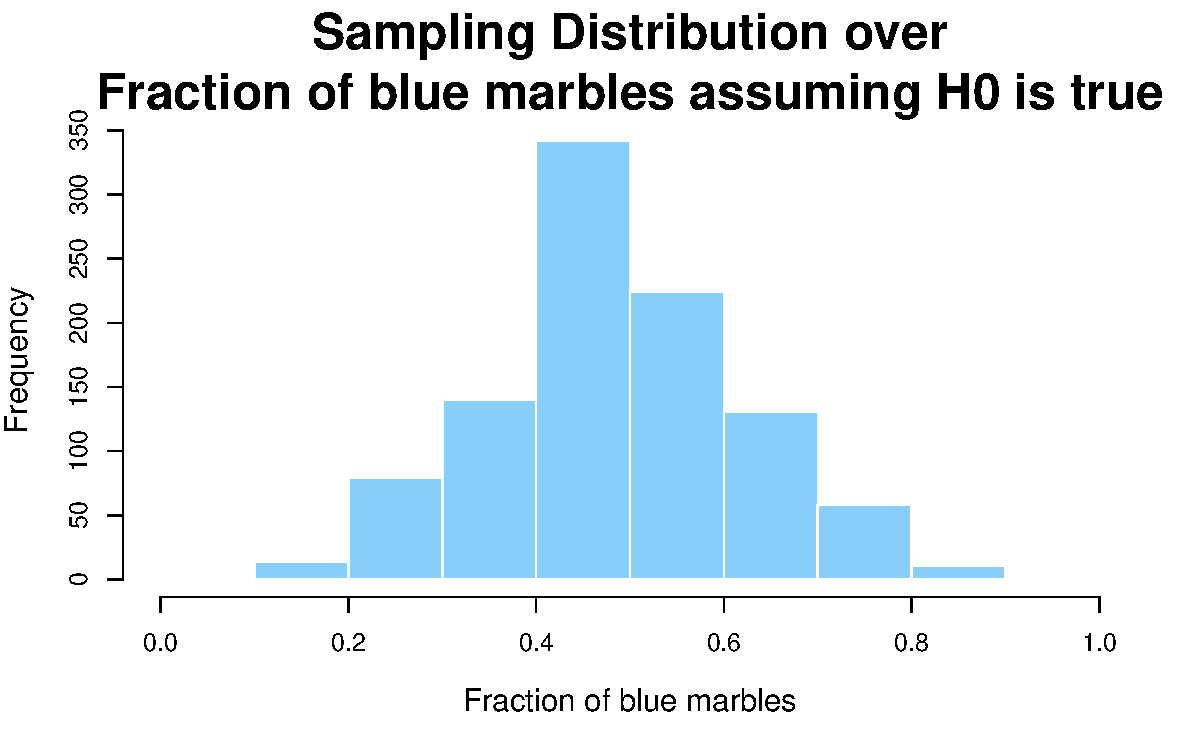
\includegraphics[scale=0.4]{null_05.pdf}
\end{center}

\end{frame}

%@@@@@@@@@@@@@@@@@@@@@@@@@@@@@@@@@@@@@@@@@@@@@@@@@
\begin{frame}
\frametitle{Null distribution}
  
\begin{itemize}
\item \textbf{Remember the marbles in the bag?}  We didn't talk about it but our test statistic was the fraction of blue marbles in the sample;
\bigskip

\item Imagine when we did that our null hypothesis was that the fraction of blue marbles $=$ 33\%.  Then the sampling (null) distribution ought to look like:
\end{itemize}

\begin{center}
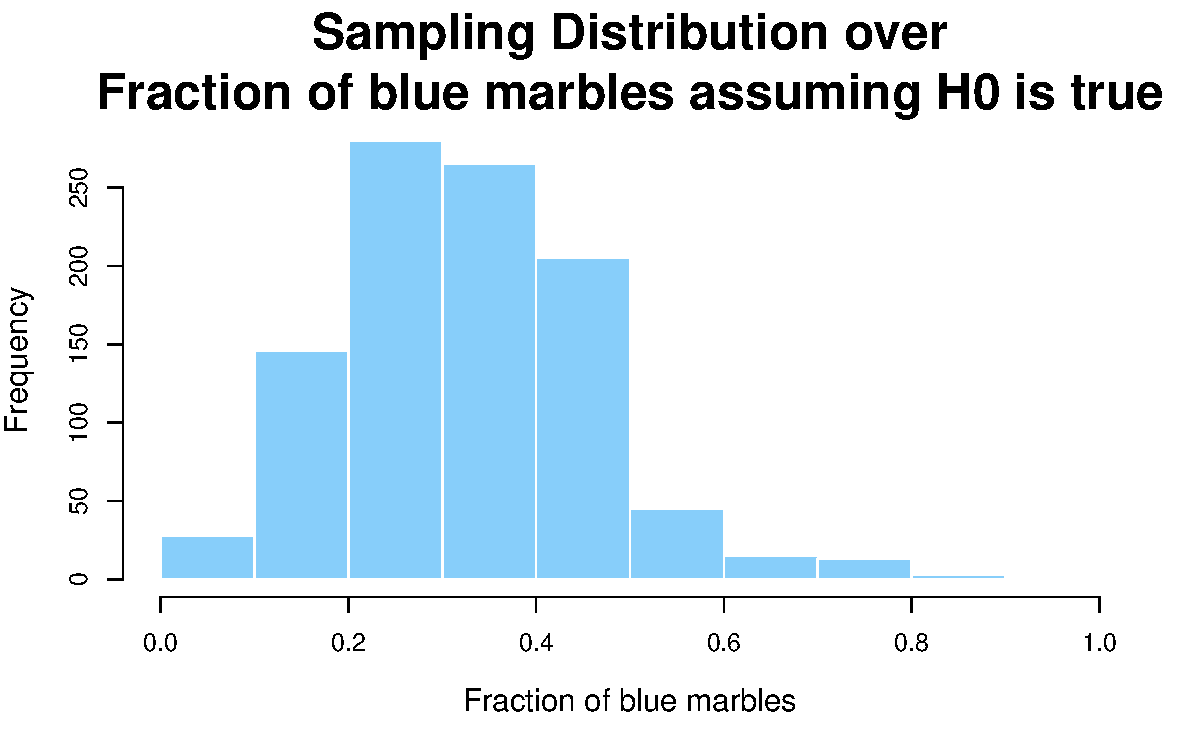
\includegraphics[scale=0.4]{null_03.pdf}
\end{center}

\end{frame}

%@@@@@@@@@@@@@@@@@@@@@@@@@@@@@@@@@@@@@@@@@@@@@@@@@
\begin{frame}
\frametitle{Null distribution}
  
\begin{itemize}
\item \textbf{Remember the marbles in the bag?}  We didn't talk about it but our test statistic was the fraction of blue marbles in the sample;
\bigskip

\item Imagine when we did that our null hypothesis was that the fraction of blue marbles $=$ 0\%.  Then the sampling (null) distribution ought to look like:
\end{itemize}

\begin{center}
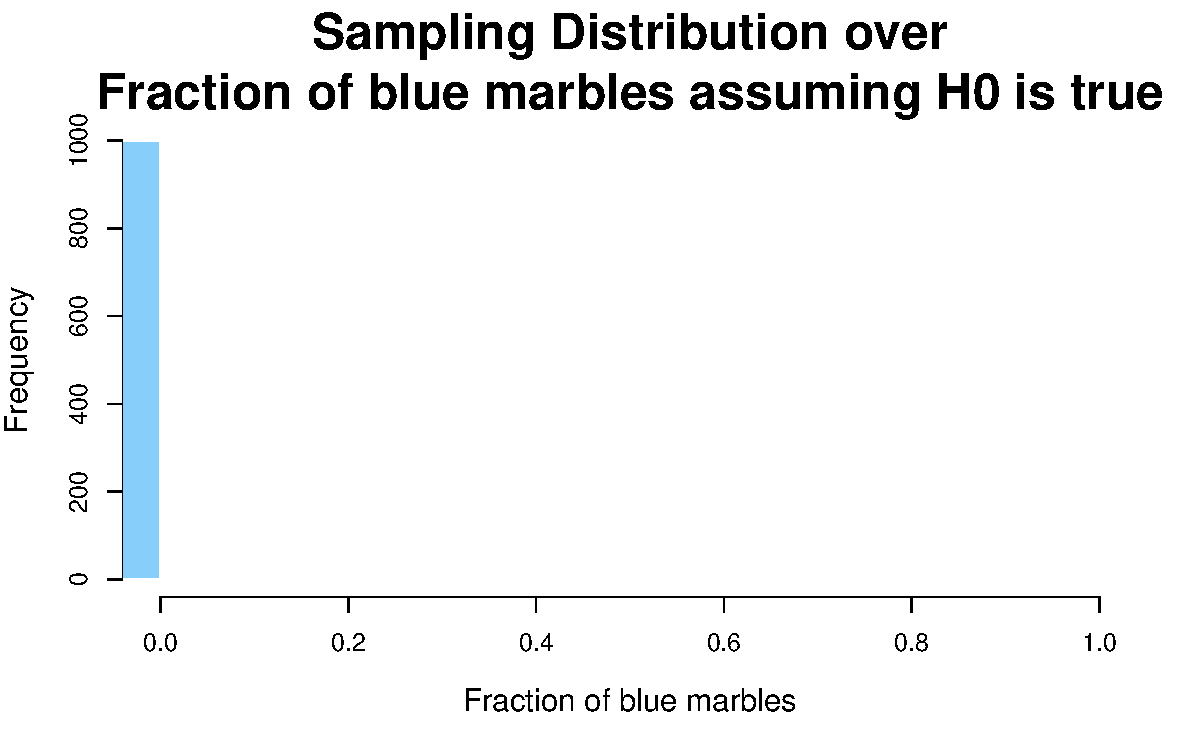
\includegraphics[scale=0.4]{null_0.pdf}
\end{center}

\end{frame}

%@@@@@@@@@@@@@@@@@@@@@@@@@@@@@@@@@@@@@@@@@@@@@@@@@
\begin{frame}
\frametitle{Choosing the rejection criterion: Type I errors and $p$-values}

\begin{itemize}
\item A \textbf{type I error} is when we reject $H_0$ when it is true;
\begin{itemize}
\item This would mean mistakenly endorsing $H_A$;
\item A similar idea is that of a false positive;
\item The probability of a type I error is usually called $\alpha$;
\end{itemize}
\bigskip
\bigskip

\item A $\mathbf{p}$\textbf{-value} is defined as the probability of getting a more extreme value than the observed test statistic given that $H_0$ is true;
\begin{itemize}
\item Measures surprise;
\item Comes from the null distribution;
\item The lower the $p$-value the lower the risk of a type I error;
\end{itemize}
\bigskip
\bigskip

\item[]\color{white} Choosing a rejection criterion or significance level is equivalent to choosing a cutoff for $\alpha$ -- by convention this is usually $0.05$:
\begin{itemize}
\item[]\color{white} We reject $H_0$ when we are sufficiently unlikely to be making a type I error.
\item[]\color{white} We reject $H_0$ when the $p$-value is less than our $\alpha$ cutoff of $0.05$.
\end{itemize}
\end{itemize}

\end{frame}

%@@@@@@@@@@@@@@@@@@@@@@@@@@@@@@@@@@@@@@@@@@@@@@@@@
\begin{frame}
\frametitle{Choosing the rejection criterion: Type I errors and p-values}

\begin{itemize}
\item A \textbf{type I error} is when we reject $H_0$ when it is true;
\begin{itemize}
\item This would mean mistakenly endorsing $H_A$;
\item A similar idea is that of a false positive;
\item The probability of a type I error is usually called $\alpha$;
\end{itemize}
\bigskip
\bigskip

\item A $\mathbf{p}$\textbf{-value} is defined as the probability of getting a more extreme value than the observed test statistic given that $H_0$ is true;
\begin{itemize}
\item Measures surprise;
\item Comes from the null distribution;
\item The lower the $p$-value the lower the risk of a type I error;
\end{itemize}
\bigskip
\bigskip

\item Choosing a rejection criterion or significance level is equivalent to choosing a cutoff for $\alpha$ -- by convention this is usually $0.05$:
\begin{itemize}
\item We reject $H_0$ when we are sufficiently unlikely to be making a type I error.
\item We reject $H_0$ when the $p$-value is less than our $\alpha$ cutoff of $0.05$.
\end{itemize}
\end{itemize}

\end{frame}

%@@@@@@@@@@@@@@@@@@@@@@@@@@@@@@@@@@@@@@@@@@@@@@@@@
\begin{frame}
\frametitle{Applying this to reason about voters...}

\begin{columns}
\begin{column}{0.5\textwidth}

\begin{itemize}
\item Cavalier Johnson: a political candidate running a campaign for Mayor of Milwaukee;
\bigskip

\item Johnson's campaign claims that he will win the election -- in this case that means getting more than 50\% of votes from Milwaukee voters;
\bigskip

\item How to assess the Johnson campaign claim?  Conduct an experiment:
\begin{itemize}
\item \textbf{Sample} $n$ voters from Milwaukee;
\item Record the number of voters who will vote for Johnson.
\end{itemize}

\end{itemize}

\end{column}
\begin{column}{0.5\textwidth}
\begin{center}

\includegraphics[scale=0.4]{Johnson.png}
\end{center}
\end{column}
\end{columns}

\end{frame}

%@@@@@@@@@@@@@@@@@@@@@@@@@@@@@@@@@@@@@@@@@@@@@@@@@
\begin{frame}
\frametitle{Applying this to reason about voters -- let's build a hypothesis test}

\begin{itemize}

\item Suppose we collect a sample of $15$ voters and we see that $6$ of them plan to vote for Johnson.  Do we believe the Johnson campaign claim?
\bigskip
\bigskip

\item $H_0$: \color{white}the Johnson campaign claim is true, i.e. the fraction of voters who will vote for Johnson is $\pi = 0.5$;
\bigskip
\bigskip

\item \color{black}$H_A$: \color{white}the Johnson campaign claim is false, i.e. the fraction of voters who will vote for Johnson is $\pi<0.5$;
\bigskip
\bigskip

\item \color{black}Test statistic: \color{white} the number of Johnson voters in our sample, in this case $6$;

\end{itemize}
\end{frame}

%@@@@@@@@@@@@@@@@@@@@@@@@@@@@@@@@@@@@@@@@@@@@@@@@@
\begin{frame}
\frametitle{Applying this to reason about voters -- let's build a hypothesis test}

\begin{itemize}

\item Suppose we collect a sample of $15$ voters and we see that $6$ of them plan to vote for Johnson.  Do we believe the Johnson campaign claim?
\bigskip
\bigskip

\item $H_0$: the Johnson campaign claim is true, i.e. the fraction of voters who will vote for Johnson is $\pi = 0.5$;
\bigskip
\bigskip

\item $H_A$: the Johnson campaign claim is false, i.e. the fraction of voters who will vote for Johnson is $\pi<0.5$;
\bigskip
\bigskip

\item \color{black}Test statistic: \color{white} the number of Johnson voters in our sample, in this case $6$;

\end{itemize}
\end{frame}

%@@@@@@@@@@@@@@@@@@@@@@@@@@@@@@@@@@@@@@@@@@@@@@@@@
\begin{frame}
\frametitle{Applying this to reason about voters -- let's build a hypothesis test}

\begin{itemize}

\item Suppose we collect a sample of $15$ voters and we see that $6$ of them plan to vote for Johnson.  Do we believe the Johnson campaign claim?
\bigskip
\bigskip

\item $H_0$: the Johnson campaign claim is true, i.e. the fraction of voters who will vote for Johnson is $\pi = 0.5$;
\bigskip
\bigskip

\item $H_A$: the Johnson campaign claim is false, i.e. the fraction of voters who will vote for Johnson is $\pi<0.5$;
\bigskip
\bigskip

\item Test statistic: the number of Johnson voters in our sample, in this case $6$;

\end{itemize}
\end{frame}

%@@@@@@@@@@@@@@@@@@@@@@@@@@@@@@@@@@@@@@@@@@@@@@@@@
\begin{frame}
\frametitle{Applying this to reason about voters -- let's build a hypothesis test}

\begin{itemize}

\item Suppose we collect a sample of $15$ voters and we see that $6$ of them plan to vote for Johnson.  Do we believe the Johnson campaign claim?
\bigskip
\bigskip

\item Our hypothesis test model says we reject $H_0$ if:
\begin{itemize}
\item The probability of a more extreme result than our observed test statistic assuming $H_0$ is true is less than $0.05$;
\item[]\color{white} The probability of a more extreme result than our observed test statistic according to the null distribution is less than $0.05$;
\item[]\color{white} The probability of 6 or fewer Johnson voters in our sample according to the null distribution is less than $0.05$;
\item[]\color{white} The $p$-value is less than $0.05$;
\end{itemize}
\bigskip
\bigskip

\item[]\color{white} So what is the probability of 6 or fewer Johnson voters in our sample?  It would be:
\begin{align*}
[]\color{white}p(0& \mbox{ Johnson voters}) + p(1 \mbox{ Johnson voter}) + p(2 \mbox{ Johnson voters})\\
[]\color{white}&p(3 \mbox{ Johnson voters}) + p(4 \mbox{ Johnson voters}) + p(5 \mbox{ Johnson voters})\\
[]\color{white}& + p(6 \mbox{ Johnson voters}).
\end{align*}

\end{itemize}

\end{frame}

%@@@@@@@@@@@@@@@@@@@@@@@@@@@@@@@@@@@@@@@@@@@@@@@@@
\begin{frame}
\frametitle{Applying this to reason about voters -- let's build a hypothesis test}

\begin{itemize}

\item Suppose we collect a sample of $15$ voters and we see that $6$ of them plan to vote for Johnson.  Do we believe the Johnson campaign claim?
\bigskip
\bigskip

\item Our hypothesis test model says we reject $H_0$ if:
\begin{itemize}
\item The probability of a more extreme result than our observed test statistic assuming $H_0$ is true is less than $0.05$;
\item The probability of a more extreme result than our observed test statistic according to the null distribution is less than $0.05$;
\item[]\color{white} The probability of 6 or fewer Johnson voters in our sample according to the null distribution is less than $0.05$;
\item[]\color{white} The $p$-value is less than $0.05$;
\end{itemize}
\bigskip
\bigskip

\item[]\color{white} So what is the probability of 6 or fewer Johnson voters in our sample?  It would be:
\begin{align*}
[]\color{white}p(0& \mbox{ Johnson voters}) + p(1 \mbox{ Johnson voter}) + p(2 \mbox{ Johnson voters})\\
[]\color{white}&p(3 \mbox{ Johnson voters}) + p(4 \mbox{ Johnson voters}) + p(5 \mbox{ Johnson voters})\\
[]\color{white}& + p(6 \mbox{ Johnson voters}).
\end{align*}

\end{itemize}

\end{frame}

%@@@@@@@@@@@@@@@@@@@@@@@@@@@@@@@@@@@@@@@@@@@@@@@@@
\begin{frame}
\frametitle{Applying this to reason about voters -- let's build a hypothesis test}

\begin{itemize}

\item Suppose we collect a sample of $15$ voters and we see that $6$ of them plan to vote for Johnson.  Do we believe the Johnson campaign claim?
\bigskip
\bigskip

\item Our hypothesis test model says we reject $H_0$ if:
\begin{itemize}
\item The probability of a more extreme result than our observed test statistic assuming $H_0$ is true is less than $0.05$;
\item The probability of a more extreme result than our observed test statistic according to the null distribution is less than $0.05$;
\item The probability of 6 or fewer Johnson voters in our sample according to the null distribution is less than $0.05$;
\item[]\color{white} The $p$-value is less than $0.05$;
\end{itemize}
\bigskip
\bigskip

\item[]\color{white} So what is the probability of 6 or fewer Johnson voters in our sample?  It would be:
\begin{align*}
[]\color{white}p(0& \mbox{ Johnson voters}) + p(1 \mbox{ Johnson voter}) + p(2 \mbox{ Johnson voters})\\
[]\color{white}&p(3 \mbox{ Johnson voters}) + p(4 \mbox{ Johnson voters}) + p(5 \mbox{ Johnson voters})\\
[]\color{white}& + p(6 \mbox{ Johnson voters}).
\end{align*}

\end{itemize}

\end{frame}

%@@@@@@@@@@@@@@@@@@@@@@@@@@@@@@@@@@@@@@@@@@@@@@@@@
\begin{frame}
\frametitle{Applying this to reason about voters -- let's build a hypothesis test}

\begin{itemize}

\item Suppose we collect a sample of $15$ voters and we see that $6$ of them plan to vote for Johnson.  Do we believe the Johnson campaign claim?
\bigskip
\bigskip

\item Our hypothesis test model says we reject $H_0$ if:
\begin{itemize}
\item The probability of a more extreme result than our observed test statistic assuming $H_0$ is true is less than $0.05$;
\item The probability of a more extreme result than our observed test statistic according to the null distribution is less than $0.05$;
\item The probability of 6 or fewer Johnson voters in our sample according to the null distribution is less than $0.05$;
\item The $p$-value is less than $0.05$;
\end{itemize}
\bigskip
\bigskip

\item[]\color{white} So what is the probability of 6 or fewer Johnson voters in our sample?  It would be:
\begin{align*}
[]\color{white}p(0& \mbox{ Johnson voters}) + p(1 \mbox{ Johnson voter}) + p(2 \mbox{ Johnson voters})\\
[]\color{white}&p(3 \mbox{ Johnson voters}) + p(4 \mbox{ Johnson voters}) + p(5 \mbox{ Johnson voters})\\
[]\color{white}& + p(6 \mbox{ Johnson voters}).
\end{align*}

\end{itemize}

\end{frame}

%@@@@@@@@@@@@@@@@@@@@@@@@@@@@@@@@@@@@@@@@@@@@@@@@@
\begin{frame}
\frametitle{Applying this to reason about voters -- let's build a hypothesis test}

\begin{itemize}

\item Suppose we collect a sample of $15$ voters and we see that $6$ of them plan to vote for Johnson.  Do we believe the Johnson campaign claim?
\bigskip
\bigskip

\item Our hypothesis test model says we reject $H_0$ if:
\begin{itemize}
\item The probability of a more extreme result than our observed test statistic assuming $H_0$ is true is less than $0.05$;
\item The probability of a more extreme result than our observed test statistic according to the null distribution is less than $0.05$;
\item The probability of 6 or fewer Johnson voters in our sample according to the null distribution is less than $0.05$;
\item The $p$-value is less than $0.05$;
\end{itemize}
\bigskip
\bigskip

\item So what is the probability of 6 or fewer Johnson voters in our sample?  It would be:
\begin{align*}
p(0& \mbox{ Johnson voters}) + p(1 \mbox{ Johnson voter}) + p(2 \mbox{ Johnson voters})\\
&p(3 \mbox{ Johnson voters}) + p(4 \mbox{ Johnson voters}) + p(5 \mbox{ Johnson voters})\\
& + p(6 \mbox{ Johnson voters}).
\end{align*}

\end{itemize}

\end{frame}

%@@@@@@@@@@@@@@@@@@@@@@@@@@@@@@@@@@@@@@@@@@@@@@@@@
\begin{frame}
\frametitle{Applying this to reason about voters -- let's build a hypothesis test}

\begin{itemize}

\item Where do these probabilities come from?
\bigskip

\item[]\color{white} Remember the \textbf{binomial distribution} that models the probability of $k$ successes in $n$ trials given that each trial has probability of success $\pi$?\color{black}

\begin{align*}
p(0& \mbox{ Johnson voters}) = ???\\
p(1& \mbox{ Johnson voter}) = ???\\
p(2& \mbox{ Johnson voters}) = ???\\
p(3& \mbox{ Johnson voters}) = ???\\
p(4& \mbox{ Johnson voters}) = ???\\
p(5& \mbox{ Johnson voters}) = ???\\
p(6& \mbox{ Johnson voters}) = ???
\end{align*}

\end{itemize}

\end{frame}

%@@@@@@@@@@@@@@@@@@@@@@@@@@@@@@@@@@@@@@@@@@@@@@@@@
\begin{frame}
\frametitle{Applying this to reason about voters -- let's build a hypothesis test}

\begin{itemize}

\item Where do these probabilities come from?  Well, from the null distribution.
\bigskip

\item[]\color{white} Remember the \textbf{binomial distribution} that models the probability of $k$ successes in $n$ trials given that each trial has probability of success $\pi$?\color{black}

\begin{align*}
p(0& \mbox{ Johnson voters}) = ???\\
p(1& \mbox{ Johnson voter}) = ???\\
p(2& \mbox{ Johnson voters}) = ???\\
p(3& \mbox{ Johnson voters}) = ???\\
p(4& \mbox{ Johnson voters}) = ???\\
p(5& \mbox{ Johnson voters}) = ???\\
p(6& \mbox{ Johnson voters}) = ???
\end{align*}

\end{itemize}

\end{frame}

%@@@@@@@@@@@@@@@@@@@@@@@@@@@@@@@@@@@@@@@@@@@@@@@@@
\begin{frame}
\frametitle{Applying this to reason about voters -- let's build a hypothesis test}

\begin{itemize}

\item Where do these probabilities come from?  Well, from the null distribution.
\bigskip

\item Remember the \textbf{binomial distribution} that models the probability of $k$ successes in $n$ trials given that each trial has probability of success $\pi$?\color{black}

\begin{align*}
p(0& \mbox{ Johnson voters}) = ???\\
p(1& \mbox{ Johnson voter}) = ???\\
p(2& \mbox{ Johnson voters}) = ???\\
p(3& \mbox{ Johnson voters}) = ???\\
p(4& \mbox{ Johnson voters}) = ???\\
p(5& \mbox{ Johnson voters}) = ???\\
p(6& \mbox{ Johnson voters}) = ???
\end{align*}

\end{itemize}

\end{frame}

%@@@@@@@@@@@@@@@@@@@@@@@@@@@@@@@@@@@@@@@@@@@@@@@@@
\begin{frame}
\frametitle{Applying this to reason about voters -- let's build a hypothesis test}

\begin{itemize}

\item Where do these probabilities come from?  Well, from the null distribution.
\bigskip

\item Remember the \textbf{binomial distribution} that models the probability of $k$ successes in $15$ trials given that each trial has probability of success $\pi = 0.5$?\color{black}

\begin{align*}
p(0& \mbox{ Johnson voters}) = p(k=0,n=15,\pi=0.5) \approx 0.00003\\
p(1& \mbox{ Johnson voter}) = p(k=1,n=15,\pi=0.5) \approx 0.00046\\
p(2& \mbox{ Johnson voters}) = p(k=2,n=15,\pi=0.5)\approx 0.00320\\
p(3& \mbox{ Johnson voters}) = p(k=3,n=15,\pi=0.5)\approx 0.01389\\
p(4& \mbox{ Johnson voters}) = p(k=4,n=15,\pi=0.5)\approx 0.04166\\
p(5& \mbox{ Johnson voters}) = p(k=5,n=15,\pi=0.5)\approx 0.09164\\
p(6& \mbox{ Johnson voters}) = p(k=6,n=15,\pi=0.5)\approx 0.15274
\end{align*}

\end{itemize}

\end{frame}

%\item Remember the \textbf{binomial distribution} that models the probability of $k$ successes in $n$ trials given that each trial has probability of success $\pi$?
%\bigskip
%\bigskip
%
%\item Let's use this to compute the null distribution (the distribution over the number of Johnson voters in a sample of 15 given that $H_0$ is true so that $\pi = 0.5$).
%\bigskip

%%@@@@@@@@@@@@@@@@@@@@@@@@@@@@@@@@@@@@@@@@@@@@@@@@@
%\begin{frame}
%\frametitle{An IRL example: polling in 1936...}
%
%\begin{columns}
%\begin{column}{0.5\textwidth}
%
%\begin{itemize}
%\item Blar;
%
%\item Blar;
%
%\item Blar;
%
%\end{itemize}
%
%\end{column}
%\begin{column}{0.5\textwidth}
%\begin{center}
%
\includegraphics[scale=0.3]{LD.png}
%\end{center}
%\end{column}
%\end{columns}
%
%\end{frame}

%@@@@@@@@@@@@@@@@@@@@@@@@@@@@@@@@@@@@@@@@@@@@@@@@@
\begin{frame}
\frametitle{The null distribution in our hypothesis test (comes from the Binomial)}

\begin{center}
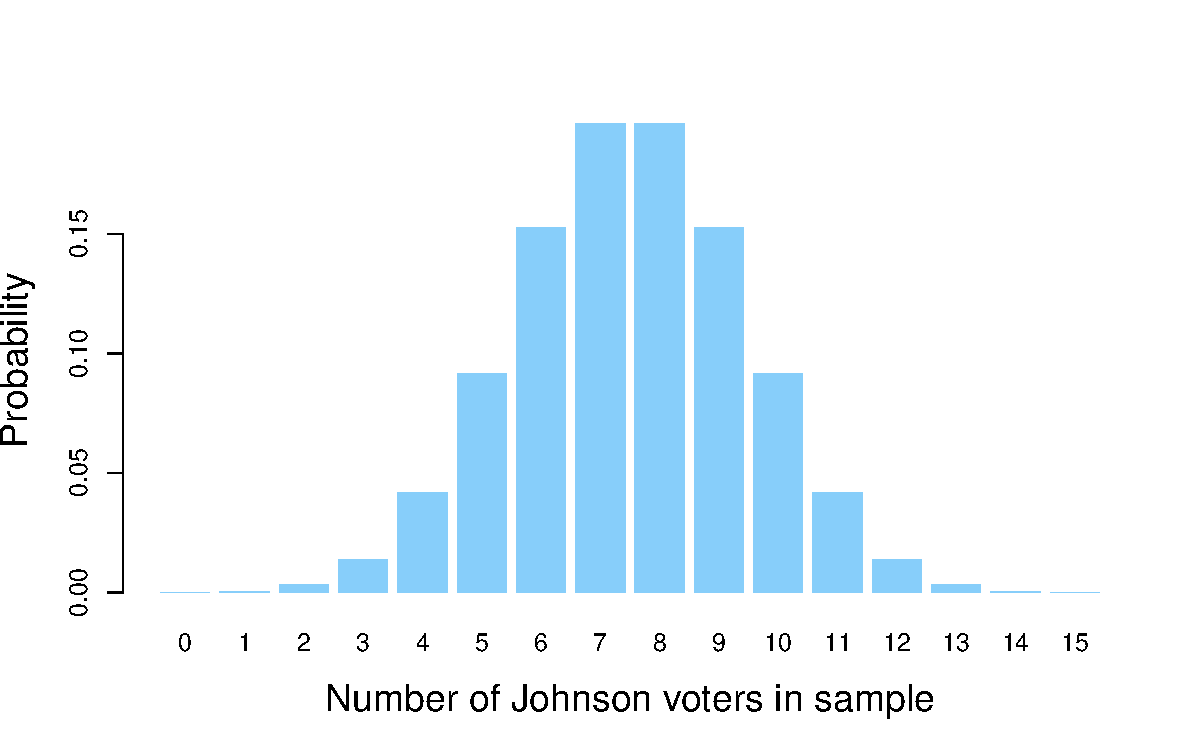
\includegraphics[scale=0.6]{binomial.pdf}
\end{center}

\end{frame}

%@@@@@@@@@@@@@@@@@@@@@@@@@@@@@@@@@@@@@@@@@@@@@@@@@
\begin{frame}
\frametitle{The null distribution in our hypothesis test (comes from the Binomial)}

\begin{center}
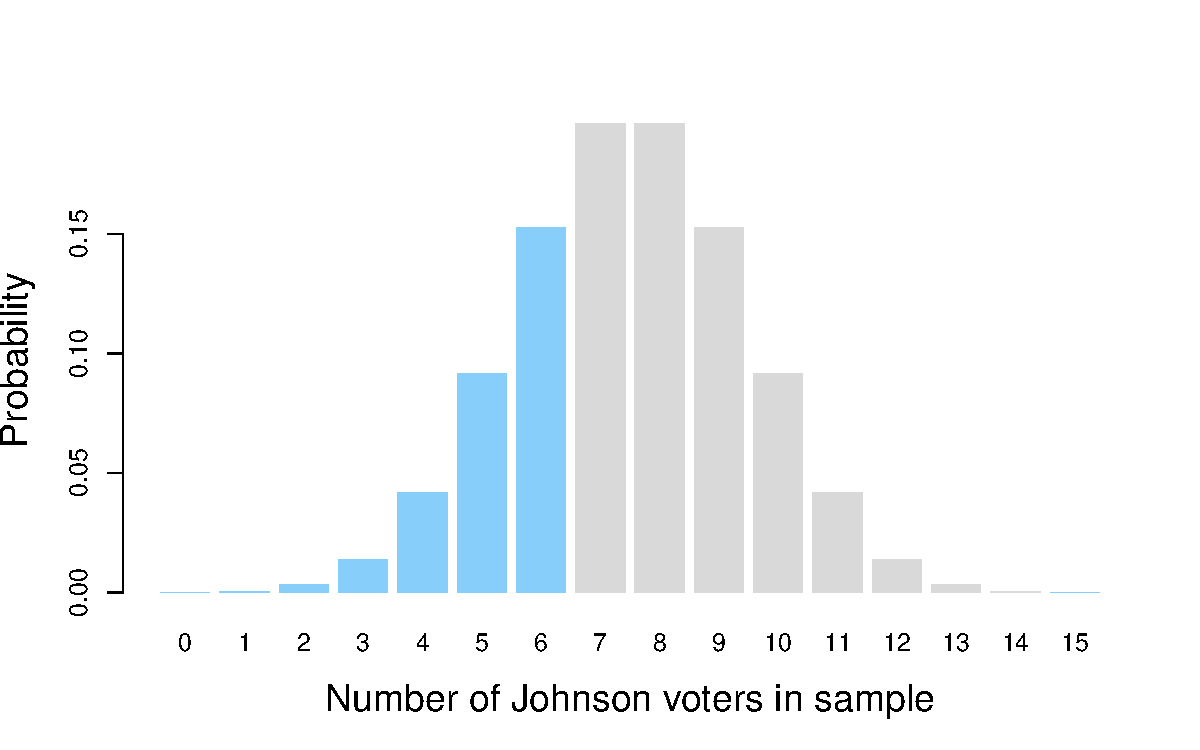
\includegraphics[scale=0.6]{binomial_2.pdf}
\end{center}

\end{frame}

%@@@@@@@@@@@@@@@@@@@@@@@@@@@@@@@@@@@@@@@@@@@@@@@@@
\begin{frame}
\frametitle{The possible $p$-values in our hypothesis test}

\begin{center}
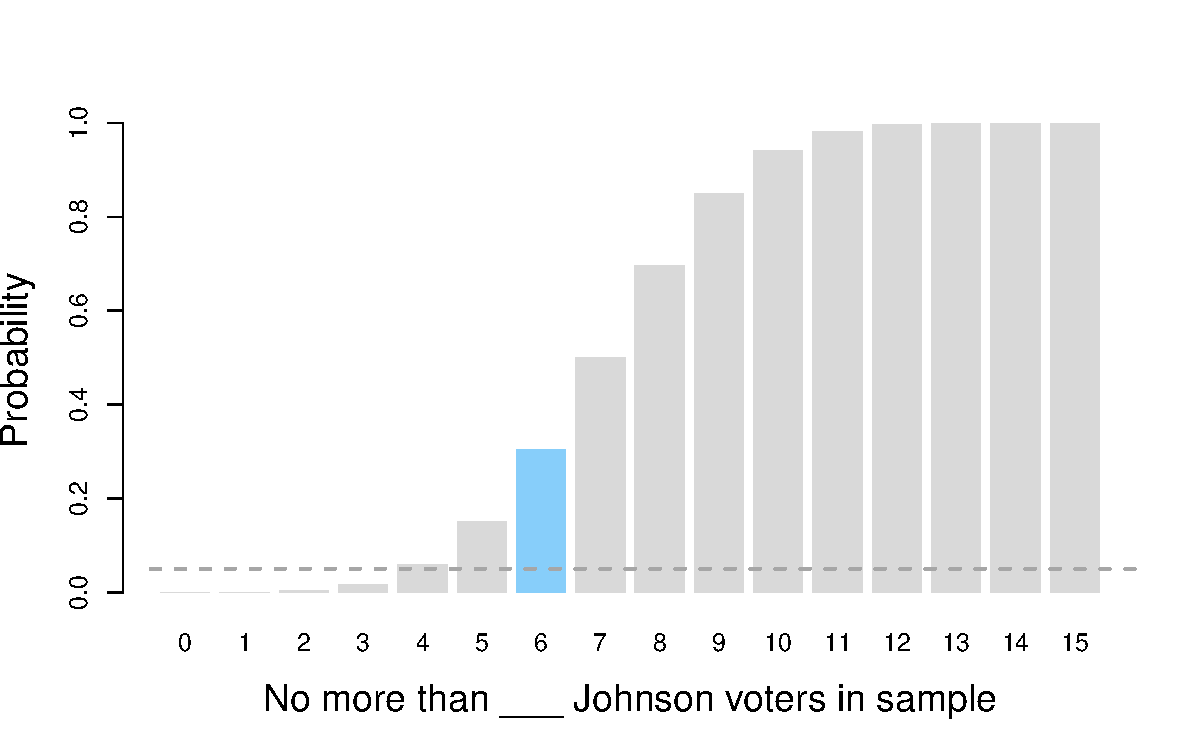
\includegraphics[scale=0.6]{binomial_CDF.pdf}
\end{center}

\end{frame}

%@@@@@@@@@@@@@@@@@@@@@@@@@@@@@@@@@@@@@@@@@@@@@@@@@
\begin{frame}
\frametitle{So...}

\begin{itemize}
\item In our Johnson voter example the $p$-value is $\approx 0.3>0.05$ meaning we fail to reject $H_0$ that Johnson will win;
\bigskip
\bigskip

\item If we had seen $4, 5,\hdots,15$ Johnson voters in our sample of $15$ the $p$-value would have been greater than 0.05 and so we would have failed to reject $H_0$ that Johnson will win;
\bigskip
\bigskip

\item If we had seen $0$, $1$, $2$, or $3$ Johnson voters in our sample of $15$ the $p$-value would have been less than 0.05 and so we would have rejected $H_0$ that Johnson will win;
\bigskip
\bigskip

\item Whenever the $p$-value $<0.05$ we would reject $H_0$.

\end{itemize}

\end{frame}

%@@@@@@@@@@@@@@@@@@@@@@@@@@@@@@@@@@@@@@@@@@@@@@@@@
\begin{frame}

\begin{center}
\Huge\textbf{Why should we care?}\\
\bigskip
\bigskip
\large Hypothesis testing is the key technique used to falsify theories in modern science.\\
\end{center}

\end{frame}



\end{document}






